

Интерполяция сплайнами - это метод интерполяции, при котором исходная функция приближается не единым полиномом на всем отрезке $[a, b]$, а семейством различных полиномов $P_{n,i}(x)$ на отрезках между узлами $[x_{i-1}, x_i]$ со сращиванием этих функций в узлах с использованием двух условий.
\begin{equation}
   S_n (x) = P_{n,i}(x), \textup{ на } [x_{i-1}, x_i]
   \label{Eq:spline_def}
\end{equation}
\begin{equation}
   S_n (x),\ S_n'(x),\ \dots,\  S_n^{(p)}(x) \textup{ непрерывны на } [a,b]
   \label{Eq:smoothness}
\end{equation}

Здесь в уравнении \eqref{Eq:spline_def} задается $S_n (x)$ - так называемая сплайн-функция или же просто сплайн. \textit{Степенью} сплайна называется максимальная степень многочленов $P_{n,i}(x)$, \textit{Степень гладкости} сплайна - количество непрерывных производных $p$ , а величина $n-p$ называется \textit{дефектом} сплайна.

Важным замечанием является то, что данный метод позволяет избежать феномена Рунге, при котором при увеличении степени интерполяционного полинома, увеличивается его ошибка в междуузлиях. Это достигается тем, что для уменьшения интерполяционной ошибки, мы увеличиваем не степень полинома, а количество отрезков.


\subsection{Линейный сплайн с дефектом 1}


Типовым примером сплайна является кусочно-линейная интерполяция или сплайн степени 1 с дефектом 1.
Он задается уравнениями
\begin{equation}
        S_1 (x)=P_{1,i} (x)=a_i+b_i (x-x_i ) \textup{ на } [x_{i-1},x_i]
\end{equation}
\begin{equation*}
        P_{1,i} (x_{i-1}) = y_{i-1},  P_{1,i} (x_i)=y_i,\ i=1 \dots n
\end{equation*}
Решая которые, получим
\begin{equation}
        P_{1,i} (x)=y_{i-1}+\frac{y_i-y_{i-1}}{x_i-x_{i-1}} (x-x_{i-1})
\end{equation}


\begin{figure}[!h]
    \centering
    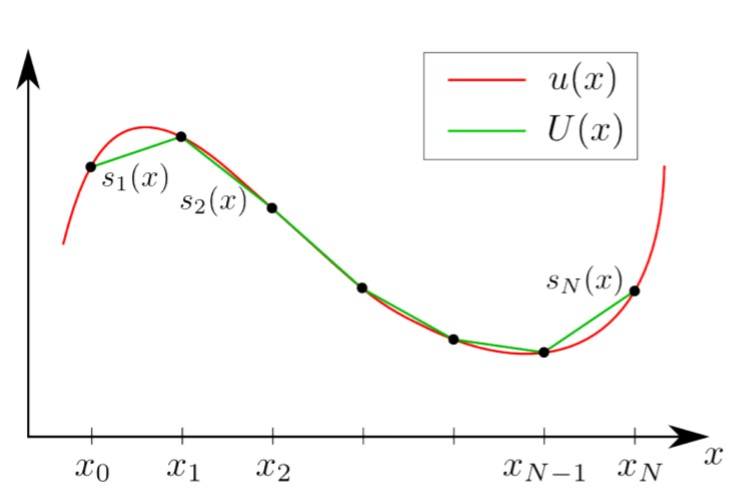
\includegraphics[width=.8\textwidth]{figures/spline_1.jpg}
    \caption{$u(x)$ - исходная функция, $U(x)$ - кусочно-линейная интерполяция}
\end{figure}